\section{L08-Cicli a vapore}
\subsection{Cicli termodinamici a vapore}
Nei cicli a vapore il fluido di lavoro subisce trasformazioni di fase.
\subsubsection{Ciclo di Carnot a vapore}
Il ciclo di Carnot è il ciclo ideale che permette di avere rendimento massimo della macchina ciclica con i serbatoi di calore che si ha a disposizione.\newline
\newline
E' composto da due isoentropiche e due isoterme (un quadrato nel diagramma temperatura e entropia).\newline
\newline
Abbiamo visto che ci sono molti svantaggi nell'impiegare il ciclo di Carnot nella versione monofase (cioè a gas): per prima cosa la trasformazione isoterma (superfici grandi e trasformazioni lente) ha caratteristiche opposte a quelle isoentropiche (superfici ridotte e trasformazioni veloci), inoltre il lavoro specifico (l'area sottesa nel diagramma pressione-volume) è molto basso.\newline
\newline
Invece, inseriamo il ciclo di Carnot all'interno di una zona bifase di una sostanza facendo corrispondere gli stati $2$ e $3$ a stati di liquido saturo e vapore saturo rispettivamente, otteniamo due isoentropiche ($1-2$ e $3-4$) e due isoterme ($2-3$ e $4-1$):
\begin{center}
    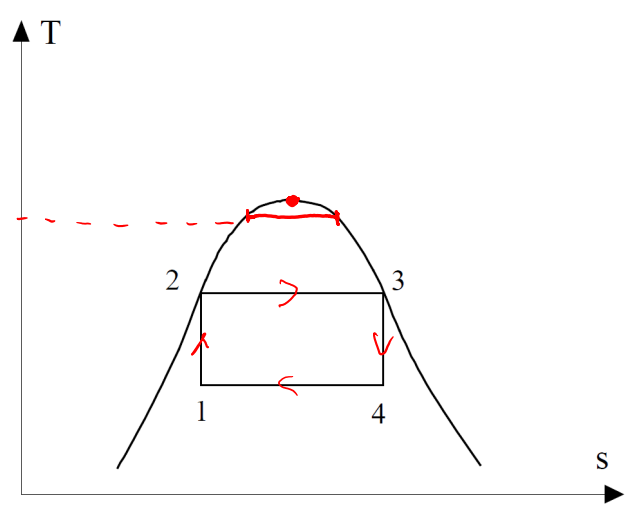
\includegraphics[height=4cm]{../L08/img1.PNG}
\end{center}
\textbf{Vantaggi}: 
\begin{itemize}
    \item Ricordiamo che se in zona bifase abbiamo temperatura costante (nelle isoterme) allora anche la pressione è costante. Ciò comporta che le isoterme siano anche isobare e dal punto di vista pratico le isobare sono facili da realizzare nella realtà.
    \item Un altro vantaggio di usare il ciclo di Carnot nella zona bifase è che c'è un notevole incremento di variazione di entalpia (dovuta all'entalpia di transizione), per cui se si guardasse l'area sottesa nel siagramma pressione-volume vedremmo che il lavoro specifico è alto.
\end{itemize}
\textbf{Svantaggi}:
\begin{itemize}
    \item E' molto dispendioso e difficile da realizzare la compressioen $1-2$.
    \item L'espansione $3-4$ è conveniente se il titolo $x_4 > 0,9$.
\end{itemize}
\subsubsection{Caratteristiche di un fluido di lavoro per il ciclo a vapore}
Per ridurre, a parità di potenza, la portata di fluido e quindi le dimensioni (e il costo) dell'impianto:
\begin{itemize}
    \item Elevata \textbf{massa volumica};
    \item Elevata \textbf{entalpia di transione di fase};
\end{itemize}
Al punto critico l'entalia di evaporazione è nulla:
\begin{itemize}
    \item Elevata \textbf{temperatura critica};
\end{itemize}
Evitare la presenza di una fase solida:
\begin{itemize}
    \item Temperature del \textbf{punto triplo} inferiore alla temperatura minima del ciclo;
\end{itemize}
Ridurre costi materiali e allungare ciclo di vita dell'impianto:
\begin{itemize}
    \item Fluido \textbf{non corrosivo};
\end{itemize}
Ridurre rischi ambientali:
\begin{itemize}
    \item Fluido \textbf{non tossico};
\end{itemize}
Aumentare sicurezza dell'impianto:
\begin{itemize}
    \item Fluido \textbf{chimicamente stabile};
\end{itemize}
Ridurre i costi:
\begin{itemize}
    \item Facilmente \textbf{reperibile e di basso costo};
\end{itemize}
Vapore in uscita dalla turbina con elevato titolo:
\begin{itemize}
    \item \textbf{Elevata pendenza} nel piano $T-s$ della curva limite superiore (più la curva è pendente e più il titolo allo stato $4$ sarà elevato);
\end{itemize}
Evitare infiltrazioni di gas incondensabili e conseguente necessità di apparecchiature atte al mantenimento dell'opportuno grado di vuoto (la temperatura al condensatore deve essere vicina a quella del serbatoio di calore inferiore per avere una limitazione delle irreversibilità):
\begin{itemize}
    \item \textbf{Pressione di condensazione} superiore alla pressione atmosferica;
\end{itemize}
\ \newline
\textbf{Nessun fluido} possiede tutte le proprietà citate. il fluido più adatto dipende dalle condizioni di contorno, in particolare delle temperatura delle sorgenti.\newline
\newline
\textbf{Cicli motore}: Tipicamente viene usata l'acqua che possiede le principali proprietà.\newline
\newline
\textbf{Cicli inversi (frigoriferi)}: Ci sono molti fluidi fra cui scogliere, per esempio:
\begin{itemize}
    \item Ammoniaca $NH_3$ (ma è tossico);
    \item Clorofluorocarburi (CFN o freon) (ma sono dannosi per l'ozono) (esempi: R11, R12);
    \item Clorofluoroidrocarburi (HCFC) e Fluoroidrocarburi (HFC) (sono meno dannosi per l'ozono) (esempi: R22, R123, R134a)
\end{itemize}
\ \newline
Vediamo una tabella che mostra le caratteristiche di acqua e R134a:
\begin{center}
    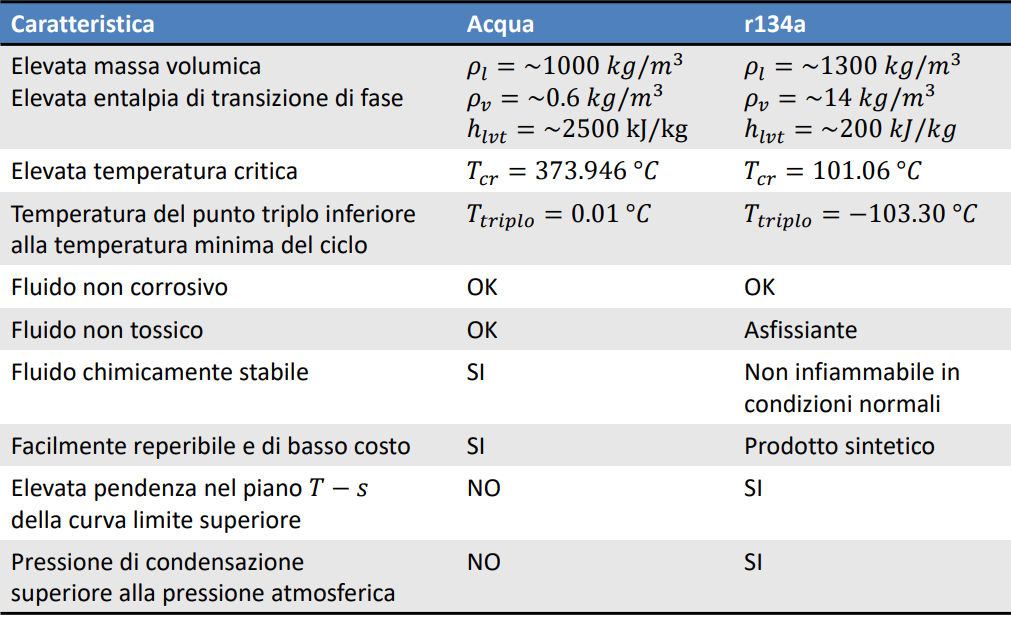
\includegraphics[height=5cm]{../L08/img2.PNG}
\end{center}
